\section{Mathematische Grundlagen}

Die Berechnungen in dieser Arbeit finden alle im reellen Raum statt, also in den
Vektorräumen $\PimiddyReell^n, n \in \{1,2,3\}$. Die Gleichungen der
Strömungsmechanik benutzen \PimiddyBegriff{Vektorfelder} und
\PimiddyBegriff{Skalarfelder}, daher sollen diese Begriffe und die zugehörigen
Operationen hier eingeführt werden.

Die später betrachteten Gleichungen sind allerdings meist gar nicht oder nur sehr
schwer analytisch zu lösen, daher greift man auf numerische Verfahren zurück.
Dafür ist es allerdings notwendig, die Operationen wie den Gradienten oder die
Divergenz zu \emph{diskretisieren}. Dies kann auf verschiedene Arten geschehen,
was im letzten Teil des Abschnitts erläutert wird.

\subsection{Kontinuierliche Felder}

Für eine Funktion $f \colon \PimiddyReell^n \to \PimiddyReell$ bezeichne

\begin{equation}
\frac{\partial f}{\partial x_i}
\end{equation}

die \PimiddyBegriff{partielle Ableitung} nach der $i$-ten Komponente.

Ein \PimiddyBegriff{Vektorfeld} $\vec{u}$ ist eine Abbildung

\begin{equation*}
\vec{u} \colon \PimiddyReell^n \to \PimiddyReell^n,
\end{equation*}

die einem Punkt im Raum einen Pfeil zuordnet. So kann z.B. jedem Punkt im Raum
die Flussgeschwindigkeit des Fluids an diesem Punkt zugeordnet werden.
\autoref{fig:mathematics_vectorfield} zeigt ein solches Vektorfeld.
$\PimiddyVectorfields(\PimiddyReell^n)$ bezeichne die Menge aller Vektorfelder.

Analog ist ein \PimiddyBegriff{Skalarfeld} $p$ eine Abbildung

\begin{equation*}
p \colon \PimiddyReell^n \to \PimiddyReell
\end{equation*}

welche einem Punkt im Raum einen skalaren Wert zuordnet. Beispielsweise könnte
für jeden Punkt im Raum die dortige Temperatur in einem Skalarfeld gespeichert
sein (siehe \autoref{fig:mathematics_scalarfield}).
$\PimiddyScalarfields(\PimiddyReell^n)$ bezeichne die Menge aller Skalarfelder.

\begin{figure}
	\begin{subfigure}[b]{0.5\textwidth}
		\centering
		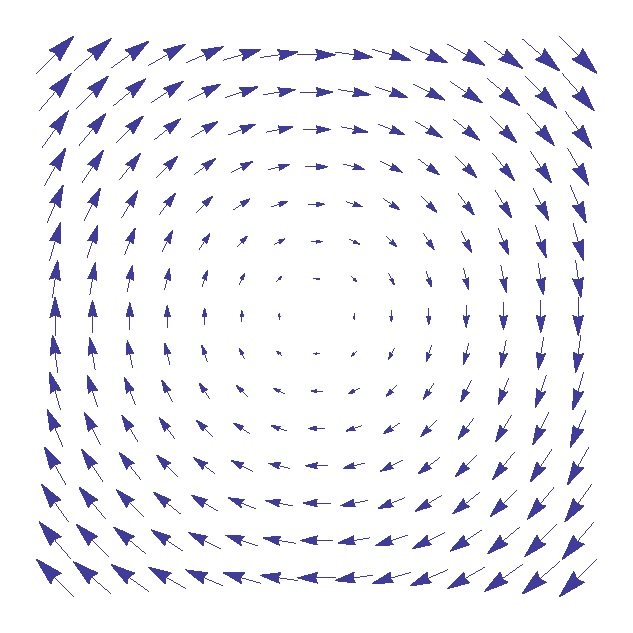
\includegraphics[width=\textwidth]{images/vectorfield}
		\caption{Ein Vektorfeld}
		\label{fig:mathematics_vectorfield}
	\end{subfigure}
	~
	\begin{subfigure}[b]{0.5\textwidth}
		\centering
		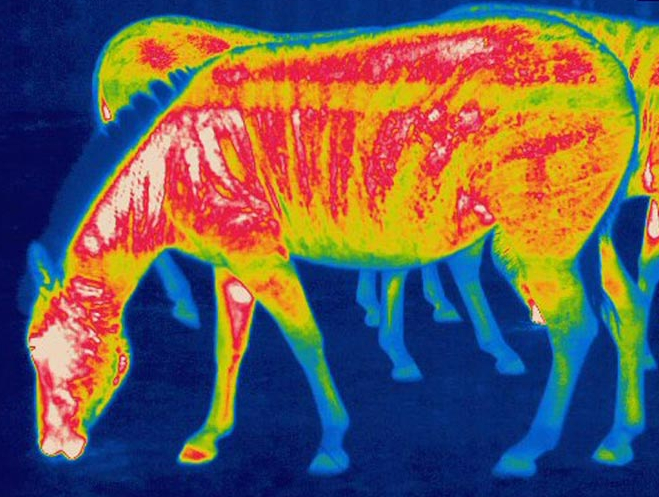
\includegraphics[width=\textwidth]{images/thermal_imaging}
		\caption{Die Körpertemparatur eines Pferds als Skalarfeld.}
		\label{fig:mathematics_scalarfield}
	\end{subfigure}
	\caption{Die betrachteten Feldtypen}
\end{figure}

Sei $p$ ein dreidimensionales Skalarfeld, dann ist der \PimiddyBegriff{Gradient}
$\PimiddyGrad p$ definiert als:

\begin{gather}
\PimiddyGrad \colon \PimiddyScalarfields \to \PimiddyVectorfields \\
\PimiddyGrad p
=
\left( \frac{\partial p}{\partial x},\frac{\partial p}{\partial y},\frac{\partial p}{\partial z} \right)
\end{gather}

\begin{figure}[ht]
	\begin{subfigure}[b]{0.5\textwidth}
		\centering
		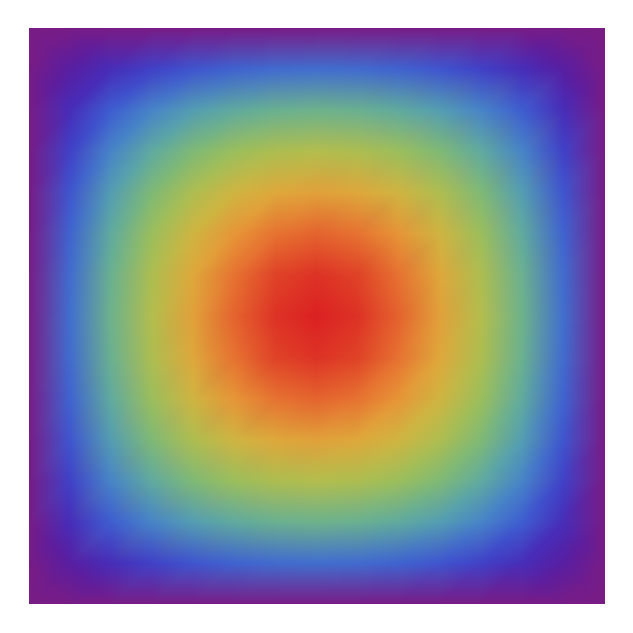
\includegraphics[width=\textwidth]{images/scalar_field_to_show_gradient}
		\caption{Das Skalarfeld zur Funktion $f(x,y) = \sin(x)\sin(y)$. Rötliche Färbung deutet hohe Werte an, lila und blau geringe.}
		\label{fig:mathematics_sample_scalar_field}
	\end{subfigure}
	~
	\begin{subfigure}[b]{0.5\textwidth}
		\centering
		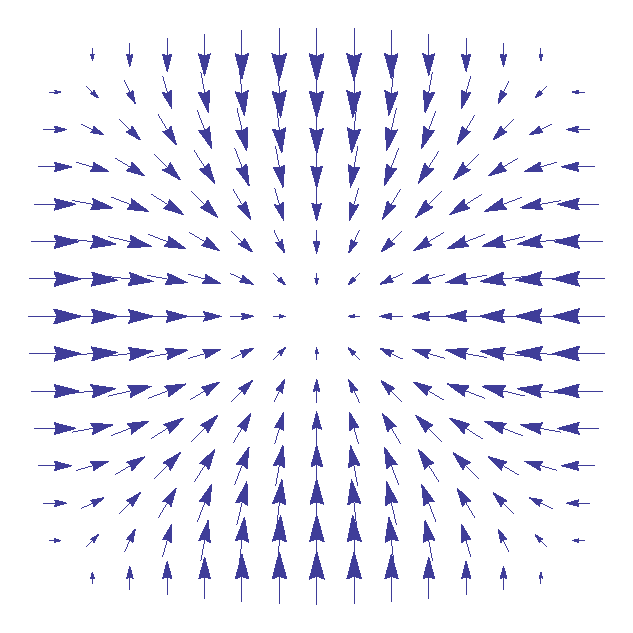
\includegraphics[width=\textwidth]{images/gradient_of_scalar_field}
		\caption{Der Gradient des Skalarfeldes $f(x,y)=(\sin(y)\cos(x),\sin(x)\cos(y))$}
		\label{fig:mathematics_gradient_of_sample_scalar_field}
	\end{subfigure}
	\caption{Der Gradient am Beispiel}
	\label{fig:mathematics_gradient_of_sample_scalar_field_total}
\end{figure}

Der Gradient eines Skalarfeldes ist also ein Vektorfeld, nämlich das Vektorfeld
der partiellen Ableitungen. Genauso wie die Ableitung eines Graphen die Steigung
an jedem Punkt angibt, so zeigt der Gradient eines Feldes in die Richtung des
steilsten Anstiegs. Seine Länge gibt die Größe Steigung an. Der Gradient des
negativen Skalarfeldes $-p$ zeigt folglich in Richtung des größten Gefälles.
\autoref{fig:mathematics_gradient_of_sample_scalar_field_total} zeigt ein simples
Beispiel für den Gradienten.

Ist ein Vektorfeld $\vec{u}$ differenzierbar (was wir in dieser Arbeit für alle
Vektorfelder annehmen), dann ist die \PimiddyBegriff{Divergenz} auf dem
Feld definiert als

\begin{gather}
\PimiddyDiv \colon \PimiddyVectorfields \to \PimiddyScalarfields \\
\PimiddyDiv \vec{u}
=
\frac{\partial u^x}{\partial x} +
\frac{\partial u^y}{\partial y} +
\frac{\partial u^z}{\partial z}
\end{gather}

Hier sind $u^x,u^y,u^z$ die einzelnen Komponenten des Vektorfeldes. Die
Divergenz eines Vektorfelds ist also ein Skalarfeld. Dieses Skalarfeld kann
gedeutet werden als \PimiddyQuotes{Quellendichte} des ursprünglichen
Vektorfeldes. Ein Feld $\vec{u}$, was $\PimiddyDiv \vec{u}=0$ erfüllt, heißt
folglich \PimiddyBegriff{quellenfrei}.

In der Physik findet man den Gradienten und die Divergenz meist unter dem Symbol
$\nabla$ vereint. Je nachdem, ob es auf ein Vektor- oder ein Skalarfeld
angewendet wird, wechselt es die Bedeutung.
%Diese Notation wird in der Arbeit bevorzugt, da man die Symbole $\PimiddyGrad$ bzw. $\PimiddyDiv$ in der Literatur zu Fluiddynamik kaum vorfindet.

Auf Vektorfeldern ist schließlich noch die \PimiddyBegriff{Rotation} definiert:

\begin{gather}
\PimiddyDiv \colon \PimiddyVectorfields \to \PimiddyVectorfields \\
\PimiddyDiv \vec{u}
=
\left(
	\begin{array}{c}
		\frac{\partial u_z}{\partial y} - \frac{\partial u_y}{\partial z} \\
		\frac{\partial u_x}{\partial z} - \frac{\partial u_z}{\partial x} \\
		\frac{\partial u_y}{\partial x} - \frac{\partial u_x}{\partial y}
	\end{array}
\right)
\end{gather}

Wie der Name schon andeutet gibt sie für jeden Punkt des ursprünglichen
Vektorfeldes an, wie stark und in welche Richtung es rotiert. Im
Zweidimensionalen ist die Rotation auch definiert, hier ist sie allerdings nur
ein Skalar, die Rotationsachse ist immer die imaginäre \PimiddyQuotes{$z$-Achse}
(in \autoref{fig:mathematics_scalarfield} wäre die Rotation überall konstant). Ein
Feld $\vec{u}$, was $\PimiddyRot \vec{u}=0$ erfüllt, heißt
\PimiddyBegriff{rotationsfrei}.

\begin{figure}
	\begin{subfigure}[b]{0.5\textwidth}
		\centering
		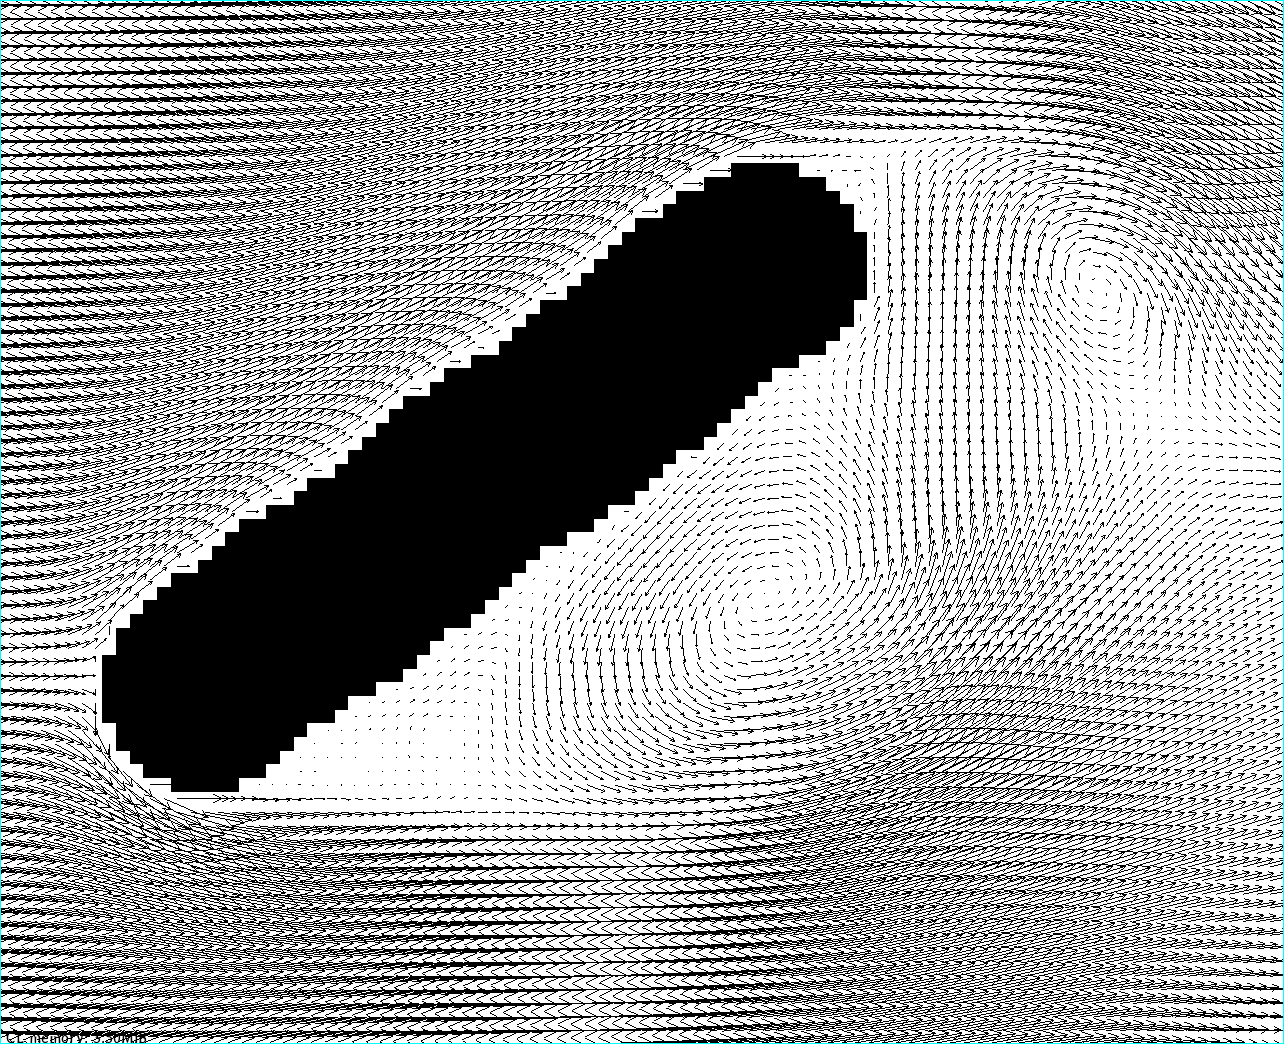
\includegraphics[width=\textwidth]{images/vector_field_rotation_arrows}
		\label{fig:mathematics_image_vectorfield_rotation_arrows}
	\end{subfigure}
	~
	\begin{subfigure}[b]{0.5\textwidth}
		\centering
		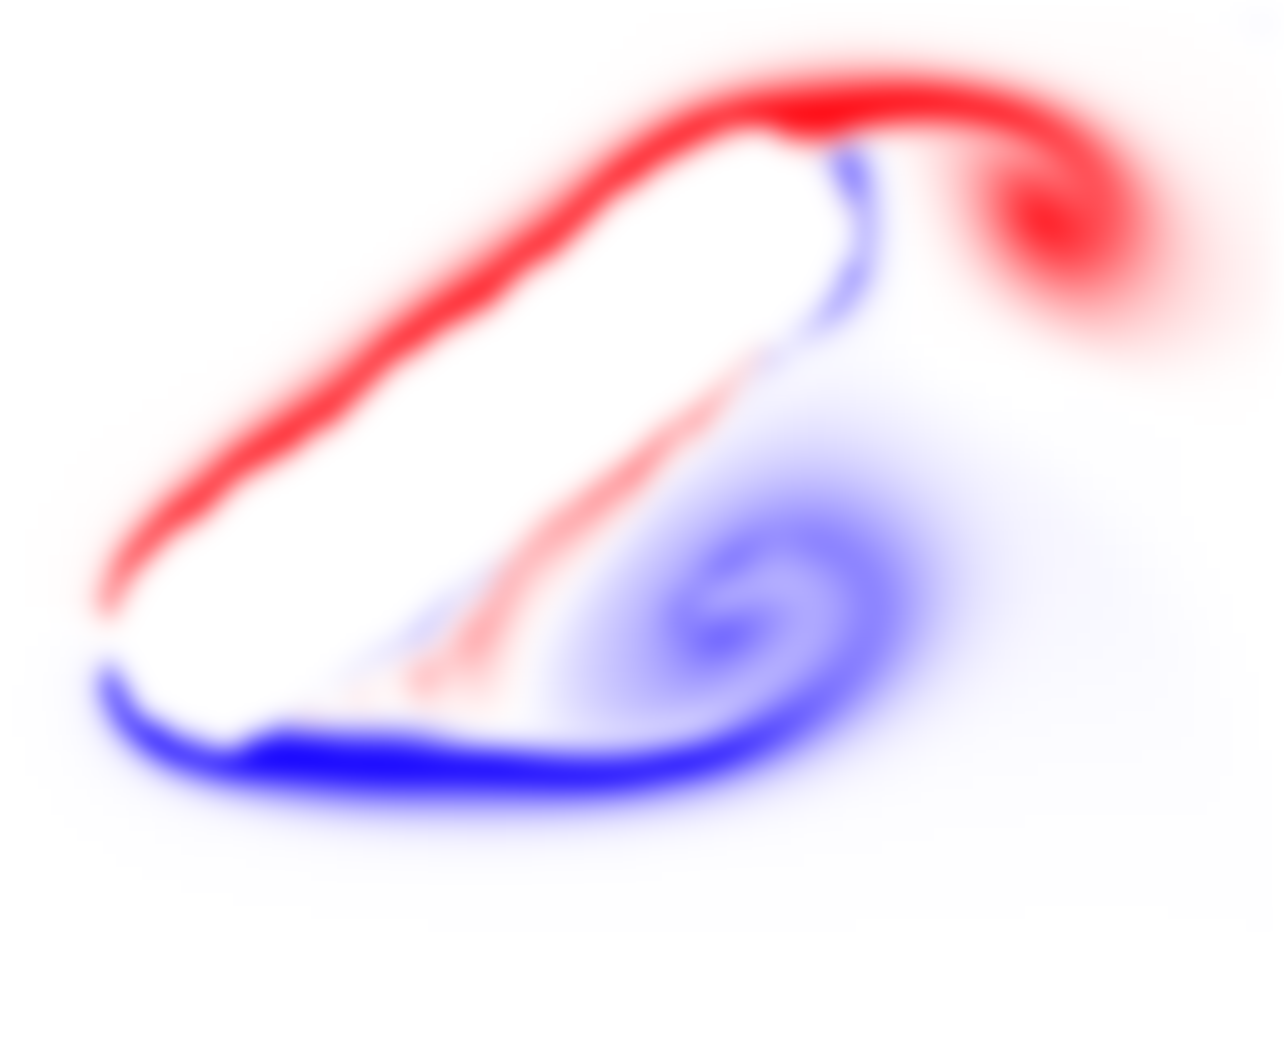
\includegraphics[width=\textwidth]{images/vector_field_rotation}
	\end{subfigure}
	\caption{Ein 2D-Strömungsfeld, das um ein Hindernis herumfließt mit dazugehöriger Rotation. Negative Rotation ist rot gekennzeichnet, positive in blau.}
\end{figure}

Schaltet man $\PimiddyGrad$ und $\PimiddyDiv$ hintereinander, erhält man den
\PimiddyBegriff{Laplace-Operator}:

\begin{gather}
\PimiddyLaplace \colon \PimiddyScalarfields \to \PimiddyScalarfields \\
\PimiddyLaplace p = \PimiddyDiv \PimiddyGrad p
\end{gather}

Manchmal wird auch das Symbol $\nabla^2$ für den Laplace-Operator benutzt. Im Dreidimensionalen ergibt sich:

\begin{equation}
\PimiddyLaplace p =
\frac{\partial^2 p}{\partial^2 x} +
\frac{\partial^2 p}{\partial^2 y} +
\frac{\partial^2 p}{\partial^2 z}
\end{equation}

Intuitiv misst der Operator für jeden Punkt $\vec{x}$ die Abweichung von
$p(\vec{x})$ zu Punkten in seiner Umgebung. Die diskretisierte Variante dieses
Operators wird deswegen in der Bildverarbeitung zum Erkennen von Kanten in
Bildern verwendet (siehe \autoref{fig:mathematics_image_laplacian}).

\begin{figure}[ht]
	\begin{subfigure}[b]{0.5\textwidth}
		\centering
		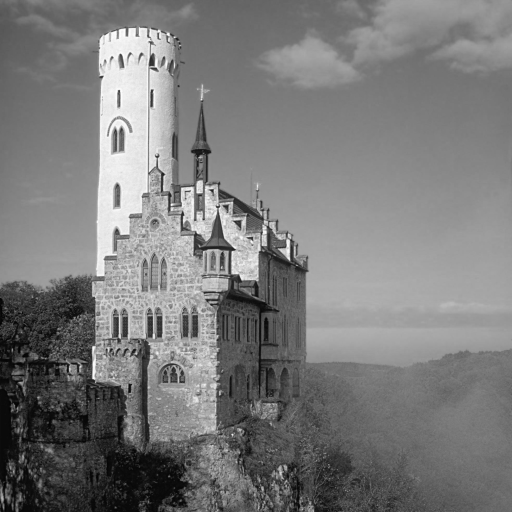
\includegraphics[width=\textwidth]{images/schloss_grey}
		\caption{Originalbild}
	\end{subfigure}
	~
	\begin{subfigure}[b]{0.5\textwidth}
		\centering
		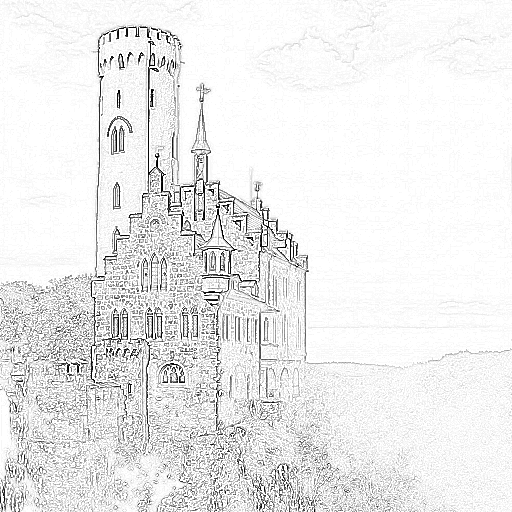
\includegraphics[width=\textwidth]{images/schloss_grey_laplace}
		\caption{Das Bild nach Anwendung des Laplace-Operators}
		\label{fig:mathematics_image_laplacian}
	\end{subfigure}
\end{figure}


Der Operator lässt sich auf nahe liegende Weise auf Vektorfelder erweitern, in drei Dimensionen
ergibt sich:

\begin{equation}
\PimiddyLaplace \vec{u} =
\left(
	\begin{array}{c}
		\PimiddyLaplace u^x \\
		\PimiddyLaplace u^y \\
		\PimiddyLaplace u^z
	\end{array}
\right)
\end{equation}

\subsection{Diskretisierung}
\label{sec:mathematics_discretization}

Die eben vorgestellten mathematischen Definitionen gehen vom unendlichen,
kontinuierlichen Raum $\PimiddyReell^n$ aus. Für die Berechnungen wird
aber ein endliches, diskretes Gitter verwendet, also eine Teilmenge von
$\PimiddyGanz^n$. Folglich müssen die Operatoren in eine diskrete Form gebracht
werden. Dies geschieht zunächst in einer Dimension.

Es sei $f \colon \PimiddyReell \to \PimiddyReell$ eine reelle Funktion, von der
wir in den späteren Berechnungen nur Stützpunkte in regelmäßigen Abständen
$\Delta x$ gegeben haben:

\begin{equation}
f_i = f(x_i) \quad , x_i = n \cdot \Delta x, n \in \PimiddyGanz
\end{equation}

Die (kontinuierliche) Ableitung dieser Funktion ist definiert als

\begin{equation}
f'(x) = \lim_{h \to 0} \frac{f(x) - f(x+h)}{x - h}
\end{equation}

Je nachdem, wie genau die Simulation sein soll, kann bei der Diskretisierung der
Ableitung unterschiedlich viel Aufwand einfließen. Grundlage für die
Diskretisierung (und die anschließende Abschätzung der Genauigkeit) ist die
\PimiddyBegriff{Taylorreihe} von $f$ (um den Entwicklungspunkt $a$):

\begin{equation}
f(x) = f(a) + f'(a)(x-a) + \frac{f''(a)}{2}(x-a)^2 + O(\Delta x^2)
\end{equation}

Nimmt man als Entwicklungspunkt $f(x_i)$ und setzt $x=x_{i+1}$ erhält man die
\PimiddyBegriff{Vorwärtsdifferenz}-Annäherung der Ableitung:

\begin{equation}
\label{eq:mathematics_forward_difference}
f'(x_i) = \frac{f(x_{i+1}) - f(x_i)}{\Delta x} + O(\Delta x)
\end{equation}

Setzt man $a=x_i,x=x_{i-1}$ erhält man analog die
\PimiddyBegriff{Rückwärtsdifferenz}:

\begin{equation}
\label{eq:mathematics_backward_difference}
f'(x_i) = \frac{f(x_i) - f(x_{i-1})}{\Delta x} + O(\Delta x)
\end{equation}

Der Nachteil dieser beiden Näherungen ist, dass sie einseitig sind (entweder
nach links oder rechts ausgerichtet) und linearen Fehler $O(\Delta x)$ haben, da
die Taylorreihe schon nach dem ersten Glied abgeschnitten wird.

Eine bessere Näherung erhält man, wenn man
\autoref{eq:mathematics_backward_difference} von
\autoref{eq:mathematics_forward_difference} subtrahiert:

\begin{equation}
f'(x_i) = \frac{f(x_{i+1}) - f(x_{i-1})}{2 \Delta x} + O(\Delta x^2)
\end{equation}

Diese Näherung wird \PimiddyBegriff{zentrale Differenz} genannt und hat
nur quadratischen Fehler $O(\Delta x^2)$. Man kann das Schema fortführen, um
noch bessere Näherung zu erhalten, dies führt allerdings dazu, dass eine immer
größere Umgebung des aktuellen Punktes betrachtet werden muss, was in der
Implementierung zu viele Speicherzugriffe verursacht.

Mit Hilfe der zentralen Differenz lässt sich auch eine Näherung für die zweite
Ableitung angeben:

\begin{equation}
f''(x_i)
=
\frac
{
	f(
		x_{i+1}) -
	2 \cdot
	f(
		x_i)
	+
	f(
		x_{i-1})
}
{
	(\Delta x)^2
}
\end{equation}

Da alle Operatoren auf partiellen Ableitungen beruhigen, lassen sich nun
diskrete Näherungen für jeden Operator angeben. Dies ist in
\autoref{table:mathematics_discrete_operator_table} für 3 Dimensionen für ein
Skalarfeld $p$ bzw. ein Vektorfeld $\vec{u}$ geschehen.

\begin{table}[ht]
	\caption{Die diskretisierten Feldoperatoren in drei Dimensionen}
	\centering
	\begin{tabular}{@{}cm{10cm}@{}}
		\toprule \\

			\PimiddyTableHeading{Operator}
		&
			\PimiddyTableHeading{Diskretisierung} \\

		\midrule \\
			$\PimiddyGrad p$
		&
			\begin{equation*}
			\frac{1}{2\Delta x}
			\begin{pmatrix}
				p_{i+1,j,k} - p_{i-1,j,k}
			\\
				p_{i,j+1,k} - p_{i,j-1,k}
			\\
				p_{i,j,k+1} - p_{i,j,k-1}
			\end{pmatrix}
			\end{equation*}
		\\
			$\PimiddyDiv \vec{u}$
		&
			\begin{equation*}
			\frac
			{
				u^x_{i+1,j,k} -
				u^x_{i-1,j,k} +
				u^y_{i,j+1,k} -
				u^y_{i,j-1,k} +
				u^z_{i,j,k+1} -
				u^z_{i,j,k-1}
			}
			{
				2\Delta x
			}
			\end{equation*}
		\\
			$\PimiddyLaplace p$
		&
			\begin{equation*}
			\frac
			{
				p_{i+1,j,k} +
				p_{i-1,j,k} +
				p_{i,j+1,k} +
				p_{i,j-1,k} +
				p_{i,j,k+1} +
				p_{i,j-1,k-1} -
				6p_{i,j}
			}
			{
				(\Delta x)^2
			}
			\end{equation*}
		\\
			$\PimiddyRot \vec{u}$
		&
			\begin{equation*}
			\frac{1}{2\Delta x}
			\begin{pmatrix}
				u^z_{i,j+1,k} - u^z_{i,j-1,k} - u^y_{i,j,k+1} + u^y_{i,j,k-1}
			\\
				u^x_{i,j,k+1} - u^x_{i,j,k+1} - u^z_{i+1,j,k} + u^z_{i,j,k-1}
			\\
				u^y_{i+1,j,k} - u^y_{i-1,j,k+1} - u^x_{i,j+1,k} + u^x_{i,j-1,k}
			\end{pmatrix}
			\end{equation*}
		\\
		\bottomrule
	\end{tabular}
	\label{table:mathematics_discrete_operator_table}
\end{table}
